\section{ER Diagram}

\begin{figure}[H] 
  \centering
  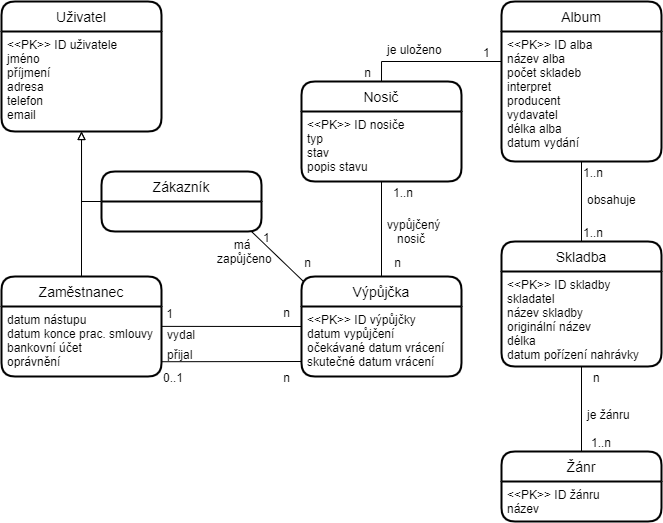
\includegraphics[scale=0.6,keepaspectratio]{er_diagram.png}
  \caption{ER Diagram}
\end{figure}


\subsection{Popis}

\subsubsection{Zákazník}
Zákazník má vypůjčeno \textbf{0 .. n} výpůjček.

\subsection{Album}
Album je uloženo na \textbf{0 .. n} nosičích (nemusí být naskladněno). \\
Album obsahuje \textbf{1 .. n} skladeb.

\subsection{Nosič}
Na nosiči je uloženo právě \textbf{1} album. \\
Nosič je by v \textbf{0 .. 1} výpůjčkách.

\subsection{Skladba}
Skladba je obsažena v \textbf{1 .. n} albech. \\
Skladba obsahuje \textbf{1 .. n} žánrů.

\subsection{Žánr}
Žánr je obsažen v \textbf{0 .. n} skladbách.

\subsection{Výpůjčka}
Výpůjčka obsahuje \textbf{1 .. n} nosičů. \\
Výpůjčce náleží \textbf{1} zákazník. \\
Výpůjčka byla vydána \textbf{1} zaměstnancem. \\
Výpůjčka byla přijata \textbf{0 .. 1} zaměstnancem.

\subsection{Zaměstnanec}
Zaměstnanec vydal \textbf{0 .. n} výpůjček. \\
Zaměstnanec přijal \textbf{0 .. n} výpůjček.